\centerline{\bf I. Introduction}
\addcontentsline{toc}{subsection}{I. Introduction}
\smallskip

\rory{get 'er done!}

\bigskip
\centerline{\bf II. Objectives and Significance}
\addcontentsline{toc}{subsection}{II. Objectives and Significance}
\smallskip

\rory{What is the point}.

\bigskip
\centerline{\bf III. Technical Approach and Methodology}
\addcontentsline{toc}{subsection}{III. Technical Approach and Methodology}
\smallskip

\medskip
{\centerline{\ub{\sc Transit Duration}}}
\smallskip

What is this definition?  Center of planet crossing?

\begin{eqnarray}
\Delta t_{circ} & = & {{P}\over{\pi}}~{{\sqrt{R_*^2 - b_0^2}}\over{a}} \nonumber \\
                & = & {{P}\over{\pi}}~{{\sqrt{1 - \beta_0^2}}\over{\alpha}}
\label{eq-tcirc}
\end{eqnarray}
where $P$ is the orbital period in cgs units, $R_*$ the stellar radius
in cgs, $b_0$ the minimum planetary impact parameter in cgs, $\beta_0$
a unitless measure of the minimum impact parameter (scaled by the
stellar radius), $a$ the planetary semi--major axis in cgs, and
$\alpha$ this value scaled by the stellar radius.


\medskip
{\centerline{\ub{\sc Fitted Transit Model}}}
\smallskip

To avoid a dependency between the fitted model and a physical model
that includes orbital dynamics, we parameterize the fitted lightcurve
in purely geometric terms.  To do so, we adopt the quadratic
limb--darkened model of \cite{2002ApJ...580L.171M}, which describes
transit lightcurves in terms of two (nuisance) limb--darkening
coefficients and two (important) system parameters.  The first of the
system parameters is the planetary radius divided by the stellar
radius ($\zeta \equiv Rp/R_*$), which determines the fractional area
of the stellar disk that may be occulted by the planet.  The second is
the impact parameter of the planet ($\beta \equiv b/R_*$).  This
variable is a function of time due to the objects' relative motion.
This function is dependent on the chord that the planet takes across
the stellar disk, itself typically estimated using the orbital
parameters semi--major axis and inclination.

Instead we use here a purely geometric parameterization, represented
in Figure~\ref{fig-schem}.  We describe the impact parameter as a
function of time using the minimum impact parameter $\beta_0$ -- when
the centers of the sources are aligned along the x--axis at
center--of--transit time $t_0$ -- and the location of the planet on
the transit chord across the stellar disk.  The x--coordinate of the
planet as a function of time is represented as $x(t) / R_* = (t - t_0)
* v_\perp / R_* = (t - t_0) / \tau$, where $v_\perp$ is the (unknown)
perpendicular velocity, and $\tau$ is the (fitted) amount of time it
takes the planet to traverse a distance equal to the stellar radius
assuming no acceleration.  This allows us to express geometrically the
impact parameter as a function of time:

\begin{eqnarray}
\beta(t) & = & \sqrt{\beta_0^2 + \left((t - t_0) / \tau\right)^2}.
\end{eqnarray}

The transit duration $\Delta t$ may be found from the 2 solutions to
$\beta(t) = 1$, and represents the time between the center of the
planet crossing each limb of the star:

\begin{eqnarray}
\Delta t & = & 2 * \tau \sqrt{1 - \beta_0^2}.
\label{eq-dt}
\end{eqnarray}
This model yields a 4--parameter fit to each transit: $t_0, \beta_0^2,
\tau, \zeta$.  The system period $P$ may be determined using the
ensemble of $t_{0;i=1...N}$.

Combining Equation~\ref{eq-dt} with Equation~\ref{eq-emin}, we express
$e_{min}$ in terms of our model parameters:
\begin{eqnarray}
e_{min} & = & \pm \frac{P^{2} - 4 \pi^{2} \alpha^{2} \tau^{2}}{P^{2} + 4 \pi^{2} \alpha^{2} \tau^{2}}
\label{eq-emin2}
\end{eqnarray}
All factors of the minimum impact parameter $\beta_0$ cancel out,
which is fortuitous as this is typically the least constrained of all
system parameters, especially for the long--cadence Kepler data.
While the uncertainty in $\beta_0$ will affect our knowledge of the
other system parameters, this uncertainty may be marginalized out by
examining the posterior distribution of system parameters, and drives
us to use Markov--Chain Monte Carlo (MCMC) modeling (described
below).

Equation~\ref{eq-emin2} indicates that $e_{min}$ is purely a function
of the fitted parameter $\tau$, the derived period $P$, and an assumed
semi--major axis for the planet (in units of the stellar radius)
$\alpha$.  The uncertainty in $e_{min}$ scales as below for all 3
parameters:

\begin{eqnarray}
\Xi & \equiv & \frac{16 \pi^{2} \alpha^{2} \tau^{2} P^{2}}{16 \pi^{4} \alpha^{4} \tau^{4} - P^{4}} \\
\delta e_{min} & = & \Xi~e_{min}~\frac{\delta \xi}{\xi} ~~~~~ \left[\xi = \tau; P; \alpha \right].\nonumber
\end{eqnarray}
In the limit of a circular orbit ($P \rightarrow 2 \pi \alpha \tau$),
$\Xi~e_{min}$ = 1.

\begin{figure*}[t] 
\begin{center} 
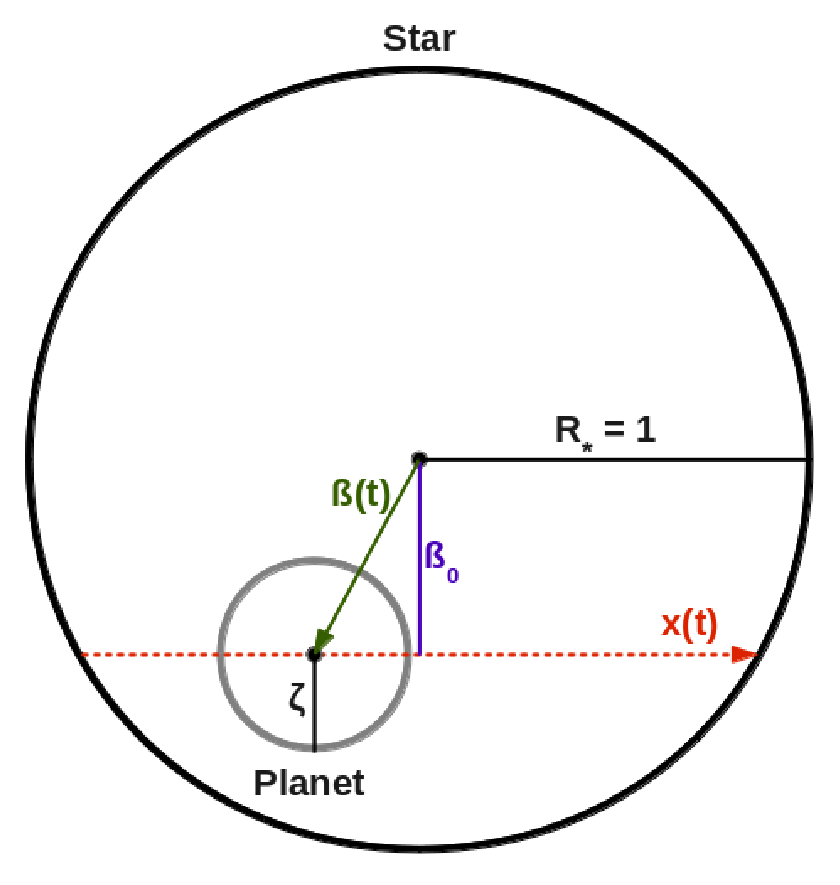
\epsfig{file=figures/schem.eps, width=0.4\textwidth} 
\caption{Schematic detailing our geometric model for the impact
  parameter as a function of time, $\beta(t)$.  Relevant variables
  include the minimum impact parameter scaled by the stellar radius
  $\beta_0$, the radius of the planet scaled by the stellar radius
  $\zeta$, and the time-dependent position of the planet $x(t)$.  The
  fitted parameters are $t_0$ (defined where $\beta(t_0) = \beta_0$),
  the minimum impact parameter $\beta_0$, scaled planetary radius
  $\zeta$, and $\tau$ (which represents the time for the planet to
  travel the angular distance subtended by the stellar radius). }
\label{fig-schem} 
\end{center} 
\end{figure*}


\medskip
{\centerline{\ub{\sc Simulations}}}
\smallskip

\rory{Describe the fake systems}

We use the system inclination, semi--major axis, planet--to--star
radius ratio, and period (along with two limb darkening parameters) to
generate fake system lightcurves using the method of
\cite{2002ApJ...580L.171M}.  The system lightcurve is evaluated once
each minute and integrated over 30 evaluations to approximate a single
Kepler long--cadence observation.  This is done for a window of 1 day
on either side of the given transit midpoint to ensure significant
out--of--transit data to include in the fit.  We perform these
evaluations for all transits for 14 ``quarters'' of Kepler
observations, or approximately 1280 days.

A white--noise component is added to each lightcurve for each of 4
magnitude bins, using the precisions in parts--per--million (ppm)
given on the Kepler calibration
webpage \footnote{http://keplergo.arc.nasa.gov/CalibrationSN.shtml}.
We evaluate each lightcurve separately for magnitude 8/10/12/14
objects, adding a random contribution of amplitude 11.3/29/80/296 ppm
(respectively) to each datapoint as generated above.  We do not
include red noise, or other transient gaps and features known to exist
in the Kepler data.  This yields a set of 4 lightcurves per simulated
system, each having hundreds of individual transits to fit.

\medskip
{\centerline{\ub{\sc Model Evaluation}}}
\smallskip

To examine how our knowledge of system parameters evolves as a
function of number of transits, we have fit the data at each transit,
using those data and data from all preceding transits.  This means
that for transit $j$, we have common model parameters $\beta_{0}^2,
\tau, \zeta$ and per--transit parameters $t_{0;1}, t_{0;2}, ...,
t_{0;j}$, for a total of $j+3$ model parameters.

We use the affine--invariant MCMC sampler {\tt emcee}
\citep{2013PASP..125..306F} to sample the posterior distribution of
the model parameters.  This program uses the method of
\cite{Goodman-Weare} to achieve high sampling performance independent
of the aspect ratio of the posterior distribution, meaning covariances
between parameters are less important to the efficacy of the MCMC
sampling.  This provides a set of MCMC chains that we examine to
determine our constraints on the fitted parameters.  We use the
Gelman--Rubin $\hat{\rm R}$--static \citep{Gelman92} to assure that
each chain sufficiently samples model space, and will require
effective chain lengths larger than $10^4$ to ensure sufficient mixing
in the MCMC sample \cite[e.g.][]{2004PhRvD..69j3501T}.  Our trial runs
using KOI 701.01 \citep[Kepler 62--b;][]{2013arXiv1304.7387B} indicate
that our chains typically have autocorrelation lengths of $\sim 100$,
requiring a total number of steps per chain of $10^6$.  This may be
achieved by using a set of $N$ {\tt emcee} ``walkers'', each taking
$10^6/N$ steps.  We will use burn--in times of $0.1 * 10^6/N$ steps,
which are then discarded before the final chain commences.  Our KOI
701.01 trials indicate that ...

For each transit, we evaluate the joint and marginalized distributions
of $\zeta$ and $\tau$.  Figure~\ref{xxx} demonstrates how the joint
distribution evolves from fitting 1 transit (dashed contours, which
represent 68.3\%, 95.5\%, and 99.7\% confidence limits), to fitting
all transits for KOI 701.01 (solid contours, at the same confidence
limit).  We then marginalize over all parameters, and examine the
confidence limits of each parameter.  Figure~\ref{fig-joint}
demonstrates how our contraints on $\zeta$ (left panel) and $\tau$
(right panel) evolve as a function of the number of transits used in
the fit.  The solid line provides the maximum of the posterior
distribution, while the dashed line indicates its median.  The shaded
area encloses 68.3\% of the distribution, i.e. 1--sigma confidence
limits.  In this way we are able to measure our unceratinty on $\tau$.

\begin{figure*}[t] 
\begin{center} 
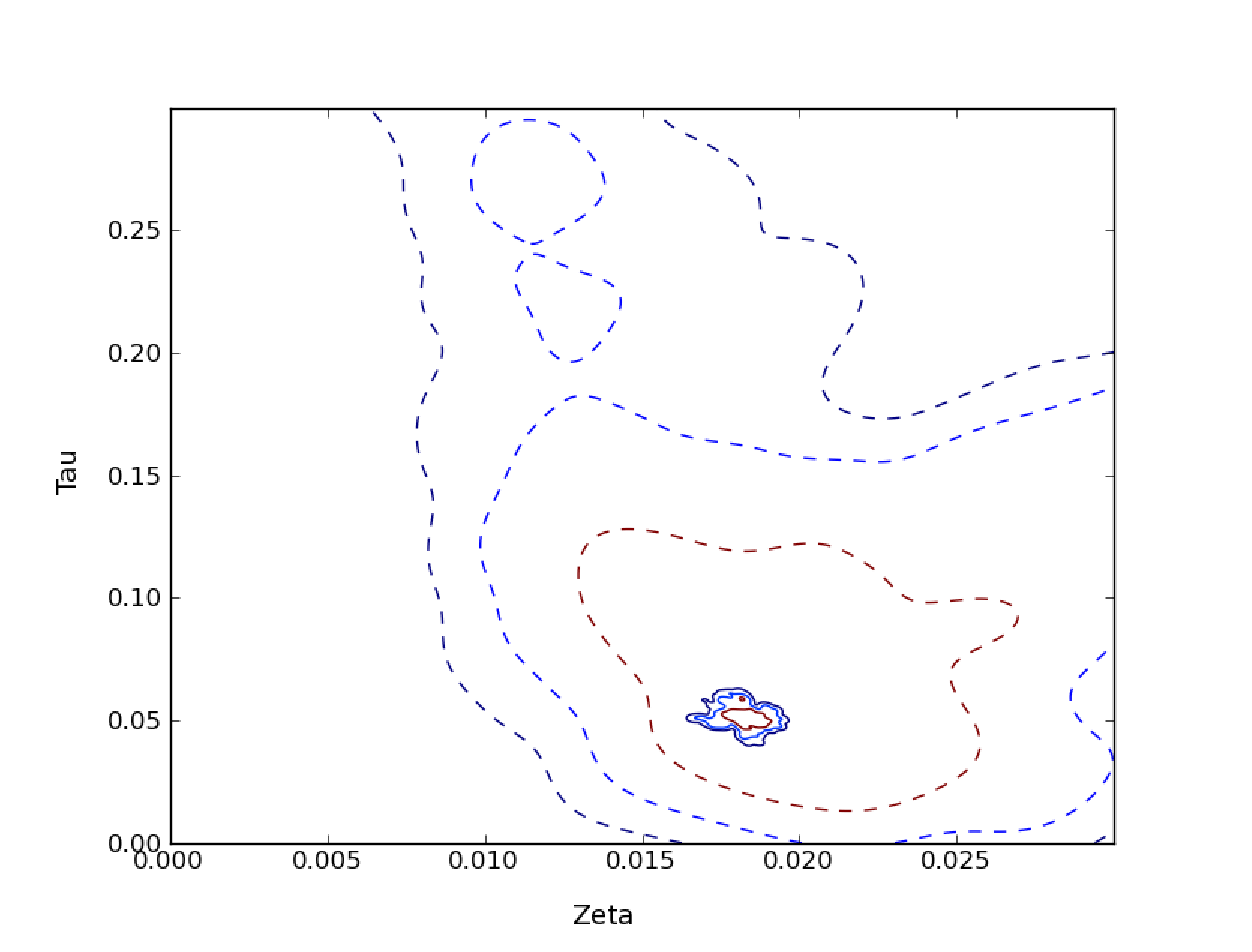
\epsfig{file=figures/joint.eps, width=0.4\textwidth} 
\caption{Joint distribution.}
\label{fig-joint} 
\end{center} 
\end{figure*}

We next examine our constraints on the system period.  We use the
posterior distributions from the fits described above for
$t_{0;1..j}$.  To do so, we use {\tt emcee} to sample the posterior
space of (nuisance parameter) $t_0$ and period $P$.  For a given trial
$t_0, P$ pair, the likelihood is determined through:
\begin{eqnarray}
\mathcal{L}(t_0, P) & = & \prod_{i=1}^{i=j} \kappa_i(t_0 + P * i)
\end{eqnarray}
where $\kappa_i$ is a kernel density estimate of each posterior
distribution $t_{0;i}$.  Figure~\ref{fig-mcmc2} shows this for the
period.  We do not fit for a linear ephemeris during the original MCMC
analysis as it precludes our modeling of a transit timing signal more
complex than $t_0 + P * i$, which may be necessary in the presence of
TTVs.

\begin{figure*}[t] 
\begin{center} 
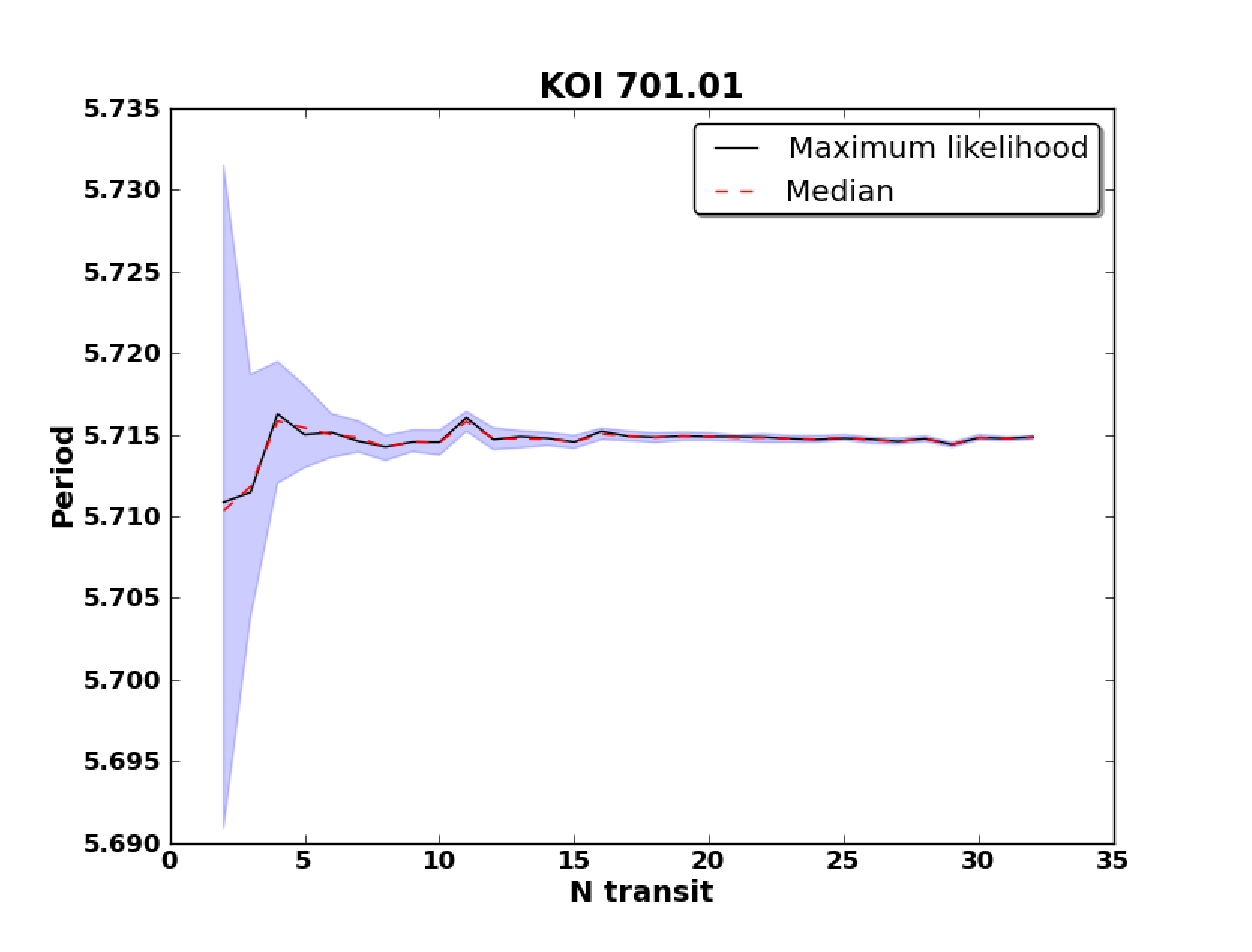
\epsfig{file=figures/period.eps, width=0.4\textwidth} 
\caption{Period.}
\label{fig-mcmc2} 
\end{center} 
\end{figure*}

We now understand how $\delta \tau$ and $\delta P$ scale.

\medskip
{\centerline{\ub{\sc Reword below}}}
\smallskip


We combine the posterior chains to determine our constraints on common
fitted terms $\tau$ and $\zeta$, both as a joint distribution and with
each marginalized over all other parameters.  We use the peak of the
distributions and the range enclosing 68.3\% of the samples to
understand our uncertainty on each parameter.  The uncertainty on
$\tau$ will feed in directly to our uncertainty on $e_{min}$ through
Equation~\ref{eq-emin2}.  Figure~\ref{fig-taurun} shows the peak value
of the $\tau$ distribution, and its uncertainty $\delta \tau$ as
described above, as a function of the number of transits sampled, for
4 magnitude bins.  Table~\ref{tab-taurun} lists the numbers of
transits that are needed to recover $\tau$ to 10\% as a function of
the system brightness and transit depth.

\begin{table}[t]
\begin{center}
\caption{\label{table-taurun} Number of transits needed to recover $\tau$ to 10\%}
\begin{tabular}{c|cccc}
\hline \hline
Transit Depth (\%) & Magnitude=8 & Mag=10 & Mag=12 & Mag=14\\
\hline
5e-5 & x & x & x & x \\
1e-4 & x & x & x & x \\
5e-4 & x & x & x & x \\
1e-3 & x & x & x & x \\
5e-3 & x & x & x & x \\
1e-2 & x & x & x & x \\
\hline
\end{tabular}
\end{center}
Estimates of the number of transits needed to recover the value of
$\tau$ to 10\%, based on our simulated systems.  We determine this as
a function of transit depth, and the signa--to--noise of the
lightcurve (here, determiend solely by the host star brightness).  We
combine all MCMC chains up to and including the transit listed here to
determine the multi--transit constraint on the distribution.
\end{table}

A bayesian estimate of the period of the system and its uncertainty is
derived from the ensemble of transit times $t_{0;i=1...N}$.  To
establish the likelihood of a trial period, we fold all MCMC steps for
$t_{0;i=1...N}$ at this period to provide an approximate posterior
distribution in orbital phase of all of the samples of
$t_{0;i=1...N}$.  This distribution will be strongly peaked when
folded at the correct period.  We create 1--dimensional kernel density
estimates (KDE) of the folded distribution, where the peak value of
the KDE reflects the likelihood of the period.  We use this peak value
of the phase distribution as the likelihood of a given period,
allowing {\tt emcee} to sample the posterior of the period
distribution.  We find that...

\begin{figure*}[t] 
\begin{center} 
\mbox{
\subfigure{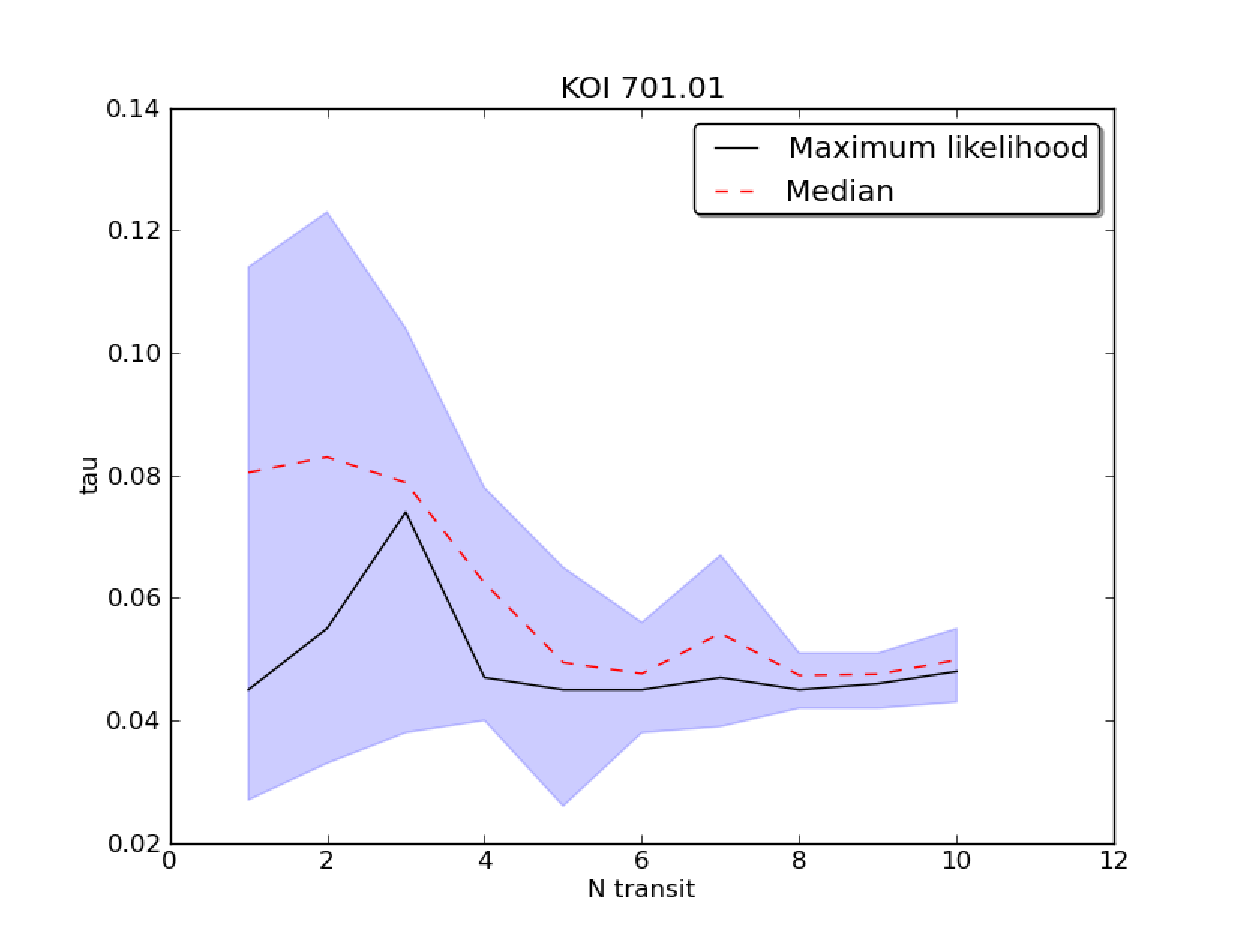
\includegraphics[width=3.3in]{figures/tau.eps}}
\quad
\subfigure{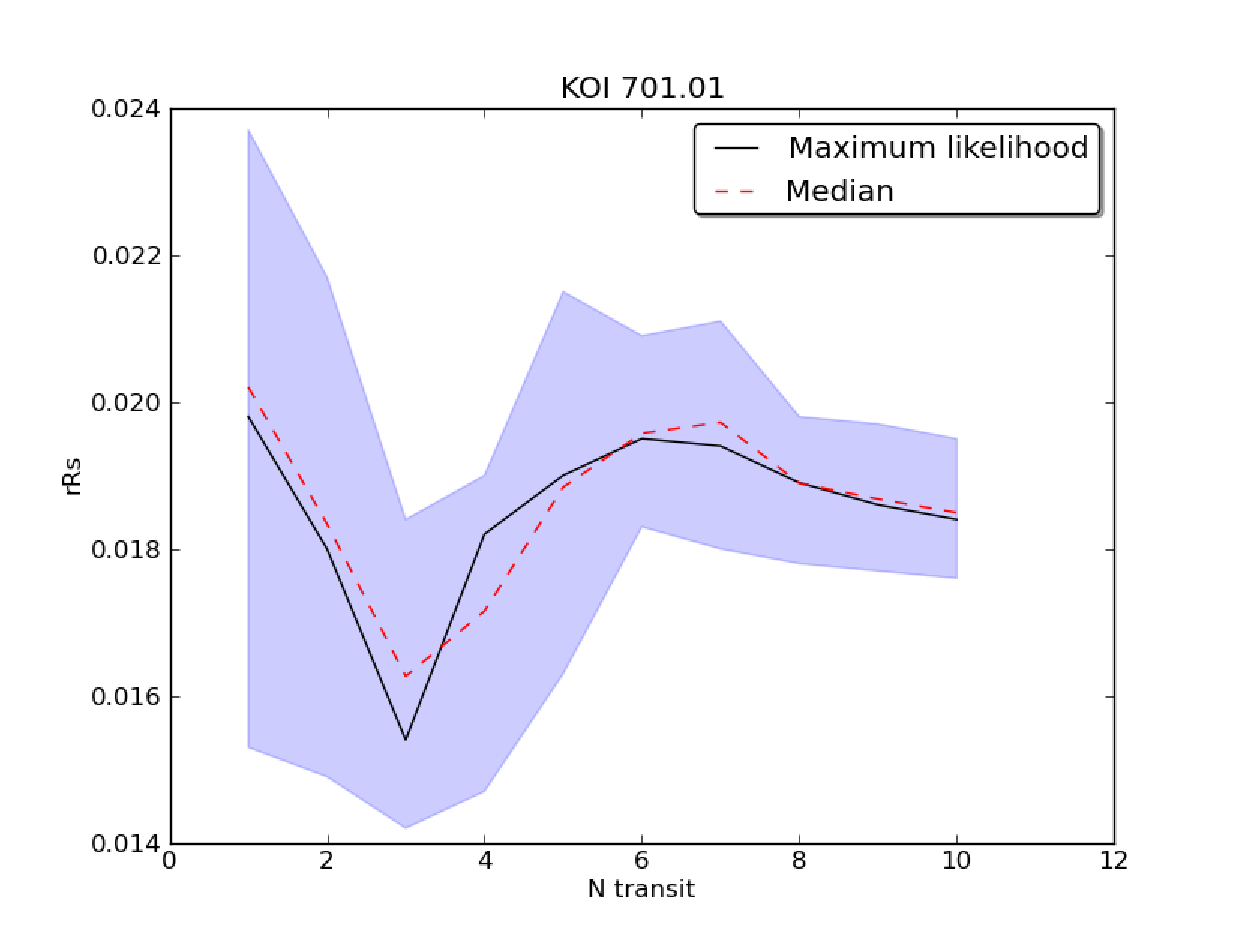
\includegraphics[width=3.3in]{figures/rRs.eps}}
}
\caption{MCMC 1}
\label{fig-mcmc1} 
\end{center} 
\end{figure*}

\medskip
{\centerline{\ub{\sc Kepler Sample Available for Analysis}}}
\smallskip

We need systems that are observed with the short cadence (ummm, maybe
not...), are bright enough to resolve $e_{min}$ to within 0.1, and
have short period planets (less than 4 days).  From this sample, we
will need to know the physical characteristics of stellar mass and
radius, and (ideally) age.

\medskip
{\centerline{\ub{\sc Computational Requirements}}}
\smallskip

For a single--threaded MCMC process using 8 walkers, each having 1000
burn--in steps that are rejected and 10000 MCMC steps that are
retained, we can fit a single transit of a single KOI in approximately
500 seconds.


\bigskip
\centerline{\bf IV. Team Qualifications and Previous NASA Support}
\addcontentsline{toc}{subsection}{IV. Team Qualifications and Previous NASA Support}
\smallskip

\bigskip
\centerline{\bf V. Relevance to NASA Programs}
\addcontentsline{toc}{subsection}{V. Relevance to NASA Programs}
\smallskip

\bigskip
\centerline{\bf VI. Project Development Plan}
\addcontentsline{toc}{subsection}{VI. Project Development Plan}
\smallskip

PI Becker will be technical lead the project for the first 1.5 years,
which will constitute the data analysis (MCMC) portion of the project.
He will work 50\% FTE with the graduate student to implement the
computations on the Kepler sample of data.  Co--I Barnes will serve as
technical lead for the project for the second 1.5 years, as the
project moves from analysis of the data to interpretation and
constraints on tidal evolution theory.  Co--I Agol has significant
experience in dealing with the Kepler data, in particular implementing
detrending algorithms to compensate for correlated noise in the Kepler
data.  He will advive as--needed throuhgout the project.

We expect the graduate student to become an expert in both areas of
this project, both the computational and modeling side and the
theoretical side.  Thus this project will develop a young graduate
student with a skillset 

{\bf Year 1 (2014):} 

{\bf Year 2 (2015):} 

{\bf Year 3 (2016):} 


\bigskip
\centerline{\bf VII. Data Sharing Plan}
\addcontentsline{toc}{subsection}{VII. Data Sharing Plan}
\smallskip
